\chapter{Funções de Green Fora do Equilíbrio \label{cap:green}}


No capítulo anterior, mostramos como a DFT pode ser utilizada para obter as propriedades eletrônicas e estruturais de sistemas no estado fundamental. Em particular, a DFT têm sido amplamente utilizada para estudar a estabilidade de estruturas de água em superfícies metálicas \cite{review_new}. No entanto, descrever a nível atomístico essas interfaces sob perturbações externas é fundamental para compreender melhor processos eletroquímicos. Assim, a descrição detalhada dessa interface é importante, pois nessa região que pode ocorrer a redistribuição de carga microscópica como resposta à alteração da voltagem aplicada \cite{review-electro}. Para isso, utilizaremos o formalismo de Funções de Green Fora do Equilíbrio (\textit{Non-Equilibrium Green's Function--NEGF}) para aplicar uma diferença de potencial e estudar os efeitos da superfície carregada sobre estruturas de água adsorvidas. Assim, nesse capítulo apresentaremos o problema investigado nesse trabalho e detalhes sobre a metodologia adotada para aplicar um potencial externo à interface água/metal.
%No capítulo anterior, mostramos como a DFT pode ser utilizada para obter as propriedades eletrônicas e estruturais de sistemas no estado fundamental. Em particular, a DFT têm sido amplamente utilizada para estudar a estabilidade de estruturas de água em superfícies metálicas \cite{review_new}. No entanto, descrever a nível atomístico essas interfaces sob perturbações externas é fundamental para compreender melhor processos eletroquímicos. Assim, a descrição detalhada dessa interface é importante, pois nessa região que pode ocorrer a redistribuição de carga microscópica como resposta à alteração da voltagem aplicada \cite{review-electro}. Para isso, utilizaremos o formalismo de Funções de Green Fora do Equilíbrio (\textit{Non-Equilibrium Green's Function--NEGF}) para aplicar uma diferença de potencial e estudar os efeitos da superfície carregada. Logo, o início desse capítulo aborda os desafios de investigar e modelar processos eletroquímicos a nível molecular -- Seção \ref{sec:EDL}. Em seguida, na Seção \ref{sec:problema} exibiremos com mais detalhes o problema investigado nesse trabalho e a metodologia adotada para investigar essa interface.%, utilizaremos Na prática, entretanto, essa descrição constitui um desafio computacional, cujos métodos disponíveis buscam o equilíbrio entre a acurácia da estrutura eletrônica e o tamanho do sistema modelado .

 
\begin{comment}
%\section{Interface Eletroquímica\label{sec:EDL}}

Uma célula eletroquímica é constituída por dois reservatórios de carga que atuam como eletrodos e separados por uma solução eletrolítica. Ao aplicar uma diferença de potencial, ocorre uma redistribuição de carga tanto na interface do eletrodo, quanto nos íons que compõem o eletrólito. Esse rearranjo leva à formação da dupla camada elétrica (\textit{electric double layer--EDL}) responsável pela formação e quebras de ligações químicas, por processos de transferências de carga e adsorção que ocorrem na interface do eletrodo \cite{electro_curcinotta}, como ilustrado na Figura \ref{fig:edl}. 

Os processos que ocorrem nessa interface estão diretamente ligados ao comportamento das moléculas de água na superfície metálica, como ilustrados na Figura \ref{fig:edl}. Consequentemente, mesmo para eletrólitos mais concentrados as moléculas de água são dominantes nessa interface. No âmbito experimental, técnicas estruturais e vibracionais têm sido utilizadas para investigar a interface água/metal ao longo das últimas décadas e revelado a dependência do comportamento das moléculas de água de acordo com o potencial externo \cite{rx1,rx2,sfg1,sfg2,sfg3,sfg_kramer,raman1,raman2}. Esse comportamento foi primeiramente observado por meio de espectroscopia de Raios-X (\textit{X-ray scattering}--XRS), o qual revelou um aumento da densidade interfacial de água em função do potencial \cite{rx1}. Além disso, \citeauthor{rx2} analisaram o efeito do potencial nas ligações de hidrogênio da interface acoplando simulações \textit{ab-initio} e espectros absorção de raios-X. 
\begin{figure}[t!]
	\centering
	\caption{Ilustração de processos que podem ocorrer na interface eletroquímica ao aplicar uma diferença de potencial: (a) ausência e (b) presença da adsorção de espécies do eletrólito no metal; reações eletroquímicas que podem levar a (c) nucleação e formação de ligações químicas das espécies adsorvidas e (d)  modificações no eletrodo.}
	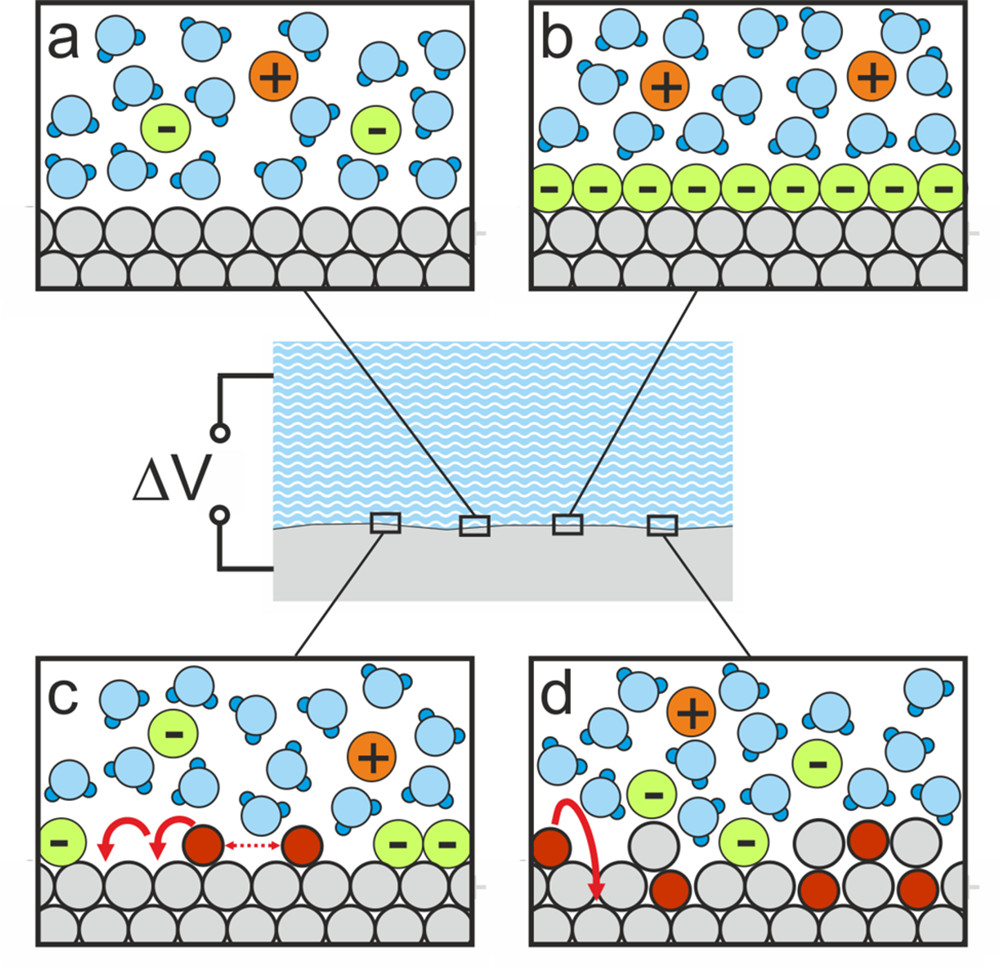
\includegraphics[scale=0.95]{figs/edl_figure.jpeg}
	\legend{Fonte: \citeauthor{edl_article}.}
	\label{fig:edl}
\end{figure}

As alterações estruturais provocadas pela variação do potencial externo é refletida nas propriedades vibracionais do sistema, como observado por meio da espectroscopia de absorção de radiação infravermelho (\textit{surface-enhanced infrared absorption spectroscopy}--SEIRAS) \cite{raman1}, o qual encontrou modificações no modo vibracional de deformação angular e um aumento do número de ligações de hidrogênio indo de potenciais negativo para positivos. Além disso, trabalhos de espectroscopia por Geração de Soma de Frequências (\textit{Sum frequency generation}--SFG), sensível somente à interface água/metal, identificou variações nas frequências mais altas de estiramento devido à variação do potencial e associaram tais modificações à ligações OH livre apontadas para o eletrodo de ouro, além de observarem uma fraca interação dessas moléculas com o metal \cite{sfg1,sfg2,sfg_kramer}. 


Em suma, resultados experimentais observam uma tendência das moléculas de se aproximarem (afastarem) do eletrodo para potenciais positivos (negativos). No entanto, os modelos experimentais ou apresentam resultados controversos sobre a estrutura da água ou são sensíveis a vibrações específicas. Isso posto, simulações computacionais são fundamentais para complementar e auxiliar na interpretação de resultados experimentais, uma vez que permite identificar estruturas cuja sensibilidade dos experimentos não captam \cite{simulacao_vibrational}. Entretanto, a modelagem computacional de processos eletroquímicos possui elevado custo, pois requerem a descrição da superfície carregada e as espécies que compõem o eletrólito e não existe uma abordagem unificada sobre como descrever tais estruturas \cite{electro_curcinotta}.


Nesse sentido, processos eletroquímicos da EDL são modelados explicitamente por meio de simulações de dinâmica molecular \textit{ab initio} ou por meio de modelos de campo médio (modelos contínuos). No primeiro caso todo o sistema é tratado atomisticamente, porém não captura corretamente efeitos eletrostáticos de longo alcance e limita o tamanho do sistema simulado \cite{review_electro}. Por outro lado, modelos contínuos representam o efeito das moléculas de água através de um meio dielétrico e não consideram a forte polarização das moléculas de água que ocorre na superfície do eletrodo \cite{hydrogen4,edl}. Isso significa que para construir modelos mais realísticos dessa interface é necessário compreender as propriedades estruturais e vibracionais da água adsorvida no metal com um potencial externo aplicado, de modo a compreender o comportamento da estrutura eletrônica da água durante o processo eletroquímico \cite{electro_curcinotta,bias_agua1}.


Na simulação eletroquímica é necessário definir o nível de aproximação através do qual os componentes da célula eletroquímica serão descritos, bem como definir o método através do qual a superfície será carregada. Um dos primeiros estudos nessa direção consistiu em simulações empíricas de dinâmica molecular clássica, no qual a eletrização da superfície metálica do eletrodo era alcançada por meio de cargas induzidas nos átomos do eletrodo \cite{charge1}. No âmbito da DFT, Neurock et. al implementou a eletrização de uma superfície metálica por meio da variação de elétrons no eletrodo e a diferença de potencial era introduzida por meio de uma camada de vácuo entre as moléculas da solução e comparado com um potencial de referência artificial (eletrodo de hidrogênio). Com essa abordagem, estudou-se a resposta da polarização da interface água/Pd(111) e água/Cu(111) em relação a um potencial externo \cite{charge2,bias-pd}. Outras implementações nesse sentido surgiram na literatura ao longo dos anos e forneceram detalhes da interface água/metal, bem como os efeitos de polarização, detalhes sobre processos que ocorrem na EDL e informações sobre energias de ativação \cite{hydrogen2,hydrogen1,hydrogen3,hydrogen4,hydrogen5}. \citeauthor{potencial1} propuseram abordar o problema acoplando o sistema a um potenciostato mantido a um potencial fixo e permitindo a troca de elétrons. Em síntese, esses modelos controlam o potencial aplicado a partir da carga adicionada ou subtraída do eletrodo, ao passo que, nos experimentos o que se controla é o potencial aplicado.

Nesse sentido, \citeauthor{artigo-luana} propuseram utilizar o formalismo de Funções de Green Fora do Equilíbrio (\textit{Non--Equilibrium Green’s Function--NEGF}) para investigar processos eletroquímicos. Com isso, os autores observaram o comportamento dependente da molécula de água em relação ao potencial externo aplicado e analisaram como a posição de mínimo é afetada pelo potencial externo. Essa abordagem permite controlar o potencial aplicado aos eletrodos sem alterar a carga total do sistema. Além disso, essa metodologia trata todos os elementos que compõem um sistema eletroquímico ao nível atomístico. Isso permite acompanhar com mais acurácia as interações e trocas de carga que ocorrem na interface entre a água e o metal. 

%Considerando a acurácia da estrutura eletrônica que essa metodologia fornece e as potenciais contribuições acerca das interações da interface água/metal, nesse capítulo abordaremos com mais detalhes esse formalismo. Iniciaremos apresentando os valores esperados de observáveis fora do equilíbrio, Seção \ref{sec:fora}; em seguida apresentaremos o formalismo de Funções de Green Fora do Equilíbrio aplicado a transporte eletrônico e, em seguida, mostraremos como esse formalismo pode ser usado para obter as propriedades eletrônicas e as forças atômicas da interface água/metal à medida que se aplica um potencial externo ao sistema. Por fim, apresentaremos o código computacional \textit{Transiesta} \cite{transiesta1}\cite{transiesta2} responsável por realizar as simulações computacionais.
 

\section{Valores Esperados de Observáveis Fora do Equilíbrio}

De modo geral, o problema de transporte eletrônico envolve um sistema no qual os eletrodos são descritos por diferentes potenciais eletroquímicos acoplados a uma região de espalhamento, o que constitui um sistema fora do equilíbrio. Para tratar problemas desse tipo, consideramos que o hamiltoniano do sistema é composto por um termo não interagente $H_0$ quadrático, um termo que descreve as interações entre partículas $H_i$ e por $H'(t)$ que representa uma pertubação aplicada ao sistema a partir de um tempo $t_0$, ou seja:
\begin{equation}\label{eq:hamiltoniano}
    \ham(t)=H_0+H_i+H'(t)
\end{equation}

Para o problema de transporte eletrônico, essa pertubação tem origem na diferença de potencial dos eletrodos. Considerando que antes da pertubação ser aplicada, o sistema esteja em equilíbrio termodinâmico com um reservatório térmico à temperatura T e um reservatório de partículas descrito por um potencial eletroquímico $\mu$, de modo que a matriz densidade do sistema no ensemble grande canônico é dado por:
\begin{equation}
    \rho(H)=\frac{e^{\beta H}}{\Tr[e^{-\beta H}]}
\end{equation}
onde $H=H_0+H_i$ e a energia das partículas foi medida em relação a $\mu=0$ por simplicidade.

Para calcular o valor esperado de observáveis para tempos $t>t_0$ de acordo com a representação de Heisenberg, tem-se:
\begin{equation}\label{eq:operador}
    \expval{O_{\ham}(t)}=\Tr[\rho(H)O_{\ham}(t)]
\end{equation}

Assim, para calcular a expressão \eqref{eq:operador}, define-se as representações de Schr\"{o}dinger e de Heisenberg de forma que elas coincidam no tempo $t_0$, isso equivale a:
$$
\ket{\Psi_{\ham}}=\ket{\Psi_S(t_0)}\quad\text{e}\quad O_{\ham}(t_0)=O_S   $$
logo, a evolução temporal de $\ham(t)$ é definida por:
\begin{equation}\label{eq:ev1}
    O_{\ham}(t)\equiv u^\dagger_{\ham}(t,t_0)O_S u_{\ham}(t,t_0)
\end{equation}
e o operador de evolução temporal é dado por:
\begin{equation}
    u_{\ham}(t,t_0)=\sum_{n=0}^{\infty}\frac{(-i)^n}{n!\hbar^n}\int_{t_0}^{t}\dd{t_1}\ldots\int_{t_0}^{t}\dd{t_n}\mathrm{T}\Bqty{\ham(t_1)\ldots\ham(t_n)}=\mathrm{T}\Bqty{e^{-\frac{i}{\hbar}\int^t_{t_0}\dd t'\ham(t')}}
\end{equation}
onde $\mathrm{T}$ é o operador de ordenamento temporal, que organiza o produtos dos operadores de acordo com suas ordens temporais, isto é, 
\begin{equation}
  \mathrm{T}\Bqty{A_1(t_1)A_2(t_2)\ldots A_n(t_n)}=(\pm1)^{P}A_{i_1}(t_{i_1})A_{i_2}(t_{i_2})\ldots A_{i_n}(t_{i_n})\;,\quad t_{i_1}>\ldots>t_{i_n}
\end{equation}
onde $P$ é o número de permutações realizadas entre os operadores em relação a ordem original, o sinal positivo corresponde a bósons e o negativo a férmions. Por outro lado, como $H=H_0+H_i$ não possui dependência temporal explícita, então a sua evolução de H é dada por:
\begin{equation}
    O_{H}(t)\equiv u^{\dagger}_H(t,t_0)O_Su_H(t,t_0)\quad\Rightarrow\quad O_S\equiv u_H(t,t_0)O_H(t)u^{\dagger}_{H}(t,t_0)
\end{equation}
onde o operador evolução temporal $u_H(t,t_0)$ é dado por:
\begin{equation}\label{eq:ev2}
    u_H(t,t_0)=e^{-i\frac{H}{\hbar}(t-t_0)}
\end{equation}

Substituindo a Equação \eqref{eq:ev1} na Equação \eqref{eq:ev1}, obtemos:
\begin{equation}\label{eq:observador}
    O_{\ham}(t)=u^{\dagger}_{\ham}(t,t_0)u_{H}(t,t_0)O_{H}(t)u^{\dagger}_H(t,t_0)u_{\ham}(t,t_0)=v^{\dagger}_H(t,t_0)O_H(t)v_H(t,t_0)
\end{equation}
onde $v_H(t,t_0)=u^{\dagger}_H(t,t_0)u_{\ham}(t,t_0)$.

Para obter o valor esperado de um operador fora do equilíbrio é conveniente remover a dependência explícita de $H'(t)$, de modo que a evolução temporal dos operadores seja governada somente por $H=H_0+H_i$. Assim, após algumas manipulações matemáticas \footnote{Os detalhes matemáticos dessas passagens podem ser consultadas em: \citetext{tese-pedro}}, o observável $O_\mathscr{H}(t)$ pode ser reescrito em termos de um operador de ordenamento de contorno $\mathrm{T}_{C_t}$, como está mostrado na Equação \eqref{eq:contorno}. Esse operador organiza o produto dos operadores de acordo com os argumentos de tempo no contorno $C_t $, que inclui os ramos do um contorno sobre o eixo real do tempo $t_0$ até $t$ e de volta a $t_0$
. 
\begin{eqnarray}\label{eq:contorno}
\mathnormal{O}_{\mathscr{H}}(t) &=& v_{\mathnormal{H}}^{\dagger}(t,t_{0})\mathnormal{O}_{\mathnormal{H}}(t)v_{\mathnormal{H}}(t,t_{0})\nonumber\\
&=&\mathrm{T}_{C_{2}}\left\{ e^{-\frac{\imath}{\hbar}\int_{C_{2}}d\tau\mathnormal{H}'_{\mathnormal{H}}(\tau)}\right\}\mathnormal{O}_{\mathnormal{H}}(t)\mathrm{T}_{C_{1}}\left\{ e^{-\frac{\imath}{\hbar}\int_{C_{1}}d\tau\mathnormal{H}'_{\mathnormal{H}}(\tau)}\right\}\nonumber\\
&=&\mathrm{T}_{C_{t}}\left\{ e^{-\frac{\imath}{\hbar}\int_{C_{t}}d\tau\mathnormal{H}'_{\mathnormal{H}}(\tau)}\mathnormal{O}_{\mathnormal{H}}(t)\right\}
\end{eqnarray}

A partir desse processo, a dependência explícita de $H'(t)$ foi removida, de modo que a evolução temporal dos operadores é governada somente por $H=H_0+H_i$. Por meio de um procedimento análogo é possível simplificar a expressão \eqref{eq:contorno} e descrevê-la somente em termos de $H_0$, de modo que a complicação em relação ao termo $H_i$, que descrevem as interações possíveis entre as partículas, é removida.
\begin{equation}
O_{\ham}(t)=\mathrm{T}_{C_t}\Bqty{ e^{-\frac{i}{\hbar}\int_{C_t}\dd\tau H^i_{H_0}(\tau) }e^{-\frac{i}{\hbar}\int_{C_t}\dd\tau H'_{H_0}(\tau)} O_{H_0}(t) }=\mathrm{T}\Bqty{S^i_{C_t}S'_{C_t}O_{H_0}(t)}
\end{equation}
onde $S^i_{C_t}=e^{-\frac{i}{\hbar}\int_{C_t}\dd\tau H^i_{H_0}(\tau) }$ e $S'_{C_t}=e^{-\frac{i}{\hbar}\int_{C_t}\dd\tau H'_{H_0}(\tau)}$.

Assim, após escrever a matriz densidade $\rho(H)$ em termos de $H_0$, o valor esperado de um observável físico fora do equilíbrio na representação de interação é dado por:
\begin{eqnarray}
\expval{\mathnormal{O}_{\mathscr{H}}(t)} &=& \dfrac{\Tr[e^{-\beta\mathnormal{H}}\mathnormal{O}_{\mathscr{H}}(t)]}{\Tr[e^{-\beta\mathnormal{H}}]} = \dfrac{\Tr[e^{-\beta\mathnormal{H}_{0}}\nu(t_{0}-\imath\hbar\beta,t_{0})\mathnormal{O}_{\mathscr{H}}(t)]}{\Tr[e^{-\beta\mathnormal{H}_{0}}\nu(t_{0}-\imath\hbar\beta,t_{0})]}\nonumber\nonumber\\
&=& \dfrac{\expval{\nu(t_{0}-\imath\hbar\beta,t_{0})\mathnormal{O}_{\mathscr{H}}(t)}_{0}}{\expval{\nu(t_{0}-\imath\hbar\beta,t_{0})}_{0}}\nonumber\\
&=& \dfrac{\expval{\mathnormal{T}_{\tilde{C}}\left\{\mathnormal{S}'_{C}\mathnormal{S}_{\tilde{C}}^{\imath}\mathnormal{O}_{\mathscr{H}}(t)\right\}}_{0}}{\expval{\mathnormal{T}_{\tilde{C}}\left\{ \mathnormal{S}'_{C}\mathnormal{S}_{\tilde{C}}^{\imath}\right\}}_{0}}
\end{eqnarray}
onde $\tilde{C}$ representa o caminho da Figura \ref{fig:contorno} e $\expval{\quad}_0$ indica que o valor esperado é calculado com respeito a $\rho(H_0)$. Esse procedimento faz com que o valor esperado dependa da matriz densidade $\rho(H_0)$ quadrática e possibilita descrever o problema fora do equilíbrio de forma diagramática. \cite{tese-pedro}
\begin{figure}[H]
	\centering
	\includegraphics[scale=0.65]{figs/contorno2.PNG}
	\caption{\textit{Contorno $\tilde{C}$ composto pelos contornos C sobre o eixo real e $C_\nu$ perpendicular ao eixo real. Fonte: \citeauthor{tese-pedro}.}}
	\label{fig:contorno}
\end{figure}  

\section{Funções de Green Fora do Equilíbrio\label{sec:fora}}

As funções de Green são definidas como as soluções de equações diferenciais inomogêneas, cuja expressão é dada por:
$$
    \bqty{z-L(\vb{r})}\green=\delta(\vb{r}-\vb{r'})
$$
sujeito à condições de contorno situadas na superfície $S$ do domínio $\Omega$ de $\vb{r}$ e $\vb{r'}$. De acordo com a notação utilizada, $z$ é uma variável complexa com $\lambda\equiv Re\Bqty{z}$ e $s\equiv Im\Bqty{z}$ e $L(\vb{r})$ é um operador diferencial linear, hermitiano e que possui um conjunto de autofunções $\Bqty{\varphi_n(\vb{r})}$ que satisfazem as mesmas condições de contorno que $\green$ \cite{green}. Para obter as propriedades das Funções de Green, é mais conveniente reescrever a equação acima utilizando a notação de Dirac:
\begin{eqnarray}\label{eq:dirac}
    \pqty{z-L}G(z)&=&\mathbb{1}\delta(z)\qquad\text{onde,}\\
    \quad\green&\equiv&\mel{\vb{r}}{G(z)}{\vb{r'}}\nonumber
\end{eqnarray}

Fora do equilíbrio, a função de Green é definida ordenada no contorno C (Figura \ref{fig:contorno}), que  se inicia em $t_0$, continua pelo eixo real, passa uma vez em $t_1$ e em $t_{1'}$ para por fim  retornar para $t_0$ e é dada pela equação:
\begin{equation}
    G(1,1')\equiv -\frac{i}{\hbar}\expval{ T_C\Bqty{ \Psi_\ham(1)\Psi^{\dagger}_\ham(1') } }
\end{equation}

onde $(1)\equiv(\vb{r}_1,\sigma_1,t_1)$ e $\Psi_\mathscr{H}$ mostra a dependência da função de onda em termos do Hamiltoniano definido na Equação \eqref{eq:hamiltoniano}. A representação de interação da Função de Green Fora do Equilíbrio é obtida de forma análoga à seção anterior, onde as grandezas envolvidas foram escritas com a dependência de $H_0$:
\begin{equation}
    G(1,1')=-\frac{i}{\hbar}\frac{\expval{T_C\Bqty{S'_CS^i_C\Psi_{H_0}(1)\Psi^{\dagger}_{H_0}(1')}  }_0 }{\expval{T_C\Bqty{S'_cS^{i}_C} }_0}
\end{equation}

\end{comment}
\section{Definindo o Problema\label{sec:problema}}

O formalismo de funções de Green fora do equilíbrio é comumente utilizado para tratar problemas de transporte eletrônico na escala atômica, no qual um objeto nanométrico situado na região central é conectado a dois reservatórios \textit{bulk} que atuam como eletrodos. Nesse arranjo, o potencial externo é aplicado por meio da diferença entre os potenciais químicos dos reservatórios. De forma análoga, uma célula eletroquímica é composta por dois eletrodos metálicos separados por uma solução eletrolítica majoritariamente composta por água. Além disso, ao aplicar uma diferença de potencial em uma célula eletroquímica o sistema fica fora do equilíbrio. Essas semelhanças permitem utilizar a abordagem de NEGF no contexto da eletroquímica para investigar atomisticamente as propriedades eletrônicas e o comportamento da molécula de água na interface com o eletrodo a diferentes potenciais como reportado por \citeauthor{artigo-luana}. 
\begin{figure}[t!]
	\centering
	\caption{Ilustração do sistema utilizado para aplicar um potencial externo sobre a interface água/metal e as regiões correspondentes aos eletrodos e região de espalhamento.}
	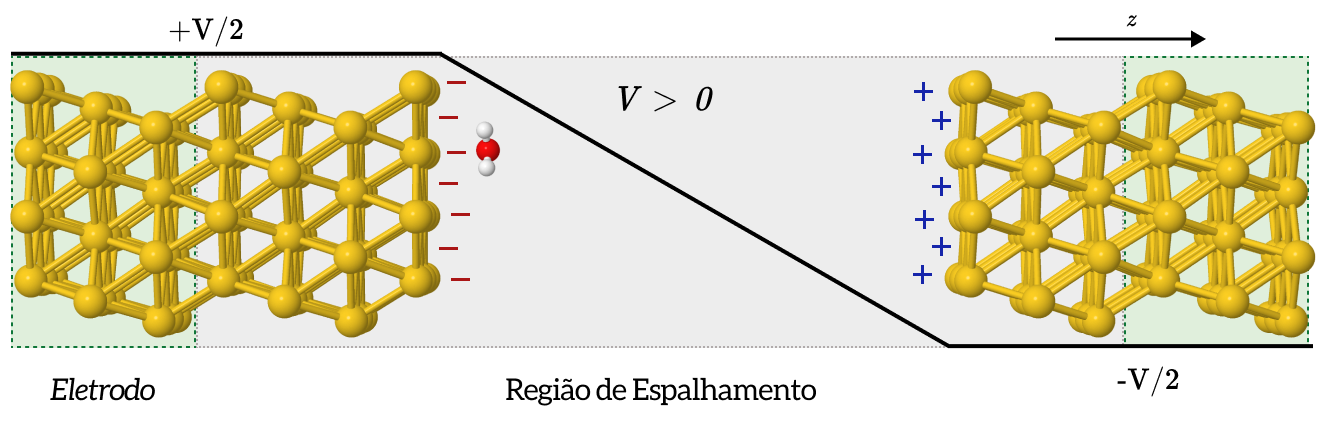
\includegraphics[scale=0.33]{figs/sistema_negf.png}
	\legend{Fonte: compilação da autora}
	\label{fig:celula}
\end{figure}

A adaptação do formalismo de NEGF a uma célula eletroquímica constitui em associar os componentes típicos da abordagem de transporte às regiões da célula eletroquímica. Assim, os reservatórios de carga correspondem aos eletrodos da célula eletroquímica e a região de espalhamento inclui algumas camadas do eletrodo metálico e a região central da célula eletroquímica, como está esquematizado na Figura \ref{fig:celula}. O sistema representado nessa imagem ilustra o protótipo de uma célula eletroquímica utilizado para investigar nesse trabalho a interface água/metal sob um potencial externo. Nessa imagem, os eletrodos são separados por uma região de vácuo e a região central da célula eletroquímica é composta por uma estrutura de água adsorvida no eletrodo esquerdo. Além disso, nessa configuração não existe fluxo de corrente pois a barreira de energia ($ \sim8 $ eV) da água é larga o suficiente para garantir que não haja fluxo, ainda que o formalismo de transporte seja capaz de tratar sistemas que tenham fluxo de corrente na região de espalhamento. Assim, esse sistema funciona como um modelo do comportamento das moléculas de água na interface sob um potencial externo aplicado e consequentemente, permite entender modelar uma  melhor os processos que ocorrem na numa célula eletroquímica.




%Do ponto de vista eletrostático, o potencial externo aplicado sobre os eletrodos produz um deslocamento de energia no espectro, ao passo que na região estendida surgirá um potencial não trivial que deve ser calculado por auto-consistência, de modo que as condições de contorno coincidam com as dos eletrodos- Figura \ref{fig:abordagem}(b). \cite{tese-alexandre}

No âmbito do formalismo de NEGF, o hamiltoniano total que descreve o sistema pode ser dividido em três partes: $H_C$ que descreve os eletrodos direito (R) e esquerdo (L), $H_T$ que representa o acoplamento entre a região central e os contatos e $H_M$ que descreve a região central onde ocorrem as interações. Tais contribuições podem ser descritos como segue abaixo:
\begin{eqnarray}
	\ham&=&(H_C^L+H_C^R)+(H_T^L+H_T^R)+H_M \\    
	H^{\alpha}_C&=&\sum_n E_{n\alpha} d^{\dagger}_{n\alpha} d_{n\alpha} \\
	H^{\alpha}_T&=&\sum_{n,k}\pqty{V_{n\alpha,k} d^{\dagger}_{n\alpha}c_k+h.c}\\
	H_M&=&H_M\pqty{\{ c^{\dagger}_k\};\{c_k\}}
\end{eqnarray}
onde $d^{\dagger}_{n\alpha}$ e $d_{n\alpha}$ são operadores de criação e destruição de um elétron no eletrodo $\alpha$ no estado n, respectivamente; ao passo que os operador $c^{\dagger}_k$/$c_k$ criam/destroem um elétron no estado k da região de interação. Os elétrons do contato são considerados não interagentes, pois os eletrodos são metálicos e estão em equilíbrio termodinâmico. Os potenciais $V_{n\alpha,k}$ dependem das densidades de cargas que são determinadas por cálculos auto consistentes. A forma do hamiltoniano $H_M$ depende do tipo de sistema que vai ser analisado.

Ao aplicar uma diferença de potencial, ocorre uma redistribuição de carga, logo é conveniente descrever o hamiltoniano em termos da densidade eletrônica. Assim, podemos descrever o sistema como uma matriz hamiltoniana e uma matriz de \textit{overlap}. Para construir os hamiltonianos dos eletrodos, consideramos que cada célula unitária que os compõem interagem somente com os primeiros vizinhos, de modo que as matrizes do hamiltonianos dos eletrodos são dadas por:
\begin{equation}
	\mathcal{H}_L =\begin{pmatrix}
		\ddots  & \vdots  & \vdots & \vdots & \vdots \\
		\ldots & H_L^0 & H_L^1 & 0 &0  \\
		\ldots & H_L^{1\dagger} & H_L^0 & H_L^1 & 0 \\
		\ldots & 0 & H_L^{1\dagger} & H_L^0 & H_L^1 \\
		\ldots & 0 & 0 & H_L^{1\dagger} & H_L^0 \\
	\end{pmatrix}\qquad 
	\mathcal{H}_R= \begin{pmatrix}
		H_R^0  & H_R^1   & 0 & 0& \ldots \\
		H_R^{1\dagger} & H_R^0 & H_R^1 & 0 &\ldots  \\
		0 & H_R^{1\dagger} & H_R^0 & H_R^1 & \ldots \\
		0 & 0 & H_R^{1\dagger} & H_R^0 & \ldots\\
		\vdots & \vdots & \vdots & \vdots & \ddots \\
	\end{pmatrix}
\end{equation}
onde o índice 0 representa a célula unitária e o índice 1 representa o acoplamento entre as células adjacentes; os subíndices R e L correspondem aos eletrodos esquerdos e direitos, respectivamente.


Para construir o hamiltoniano da região de espalhamento, adiciona-se à essa região algumas células unitárias dos eletrodos, a fim de garantir que a queda na diferença de potencial ocorra somente na parte central, de modo que a estrutura eletrônica dos eletrodos não seja alterada. Assim o hamiltoniano $\mathcal{H}$ do sistema completo é dado por:
\begin{equation}\label{eq:matriz}
\mathcal{H}=\begin{pmatrix}
\ddots & \vdots  & \vdots & \vdots & \vdots & \vdots & \iddots \\
\ldots  & H_L^0 & H_L^1 & 0 & 0 & 0 & \ldots \\
\ldots & H_L^{1\dagger} & H_L^0 & H_{LM} & 0 & 0 & \ldots \\
\ldots & 0 & H_{ML} & H_{M} & H_{MR} & 0 &\ldots  \\
\ldots & 0 &0  & H_{RM} & H_R^1 & H^1_R &\ldots  \\
\ldots & 0 & 0 & 0 & H_L^{1\dagger} & H_R^0 &\ldots \\
\iddots& \vdots & \vdots & \vdots & \vdots & \vdots & \ddots \\
\end{pmatrix}
\end{equation}
onde $H_{LM}$ e $H_{RM}$ representam o acoplamento dos eletrodos esquerdo e direito com a região de espalhamento, respectivamente. Essa matriz é infinita e não periódica.

Assim, para uma dada energia $\varepsilon$, o problema pode ser escrito em termos da função de Green retardada:
\begin{equation}
    \pqty{\varepsilon\mathcal{S}-\mathcal{H}}G^r(\varepsilon)=\mathbb{1}
\end{equation}
com $\mathcal{S}$ a matriz de overlap que segue a mesma convenção dos elementos de $\mathcal{H}$\footnote{A convenção adotada é a de que as letras caligráficas $\mathcal{H}$ e $\mathcal{S}$ representam matrizes infinitas e $H$ e $S$ matrizes finitas}. A expressão acima pode ser reescrita em termos dos hamiltonianos dos eletrodos da seguinte forma:
\begin{equation}\label{eq:matriz-esparsa}
    \begin{pmatrix}
\varepsilon\mathcal{S}_{L}-\mathcal{H}_{L} & \varepsilon\mathcal{S}_{LM}-\mathcal{H}_{LM} &0  \\
 \varepsilon\mathcal{S}_{ML}-\mathcal{H}_{ML}&\varepsilon S_{M}-H_{M}  &\varepsilon\mathcal{S}_{ML}-\mathcal{H}_{ML}  \\
0& \varepsilon\mathcal{S}_{RM}-\mathcal{H}_{RM} & \varepsilon\mathcal{S}_{R}-\mathcal{H}_{R} \\
\end{pmatrix}\begin{pmatrix}
G^r_{L} & G^r_{LM} &G^r_{LR}  \\
G^r_{ML} &G^r_{M}  & G^r_{MR} \\
G^r_{RL} &G^r_{RM}  &G^r_{R} \\
\end{pmatrix}=\mathbb{1}
\end{equation}

Como foram introduzidas no hamiltoniano da região de espalhamento algumas células unitárias dos eletrodos, essa região sentirá o efeito da interação com os eletrodos da mesma forma se tivéssemos considerando o sistema completo e com a vantagem de lidar com matrizes de dimensões finitas.

Assim, a partir da Equação \eqref{eq:matriz} podemos obter a função de Green correspondente à região de espalhamento:
\begin{equation}\label{eq:green}
    G_M^r=\pqty{\varepsilon S_M-H_M-\Sigma^{r}_L-\Sigma^{r}_R}^{-1}
\end{equation}
onde $\Sigma^{r}_L$ e $\Sigma^{r}_L$ são as autoenergias dos eletrodos esquerdo e direito, respectivamente, e são dadas por:
\begin{eqnarray}\label{eq:auto1}
\Sigma^{r}_L&=&\pqty{\varepsilon \mathcal{S}_{ML}-\mathcal{H}_{ML}}\pqty{\varepsilon \mathcal{S}_{L}-\mathcal{H}_{L}}^{-1}\pqty{\varepsilon \mathcal{S}_{LM}-\mathcal{H}_{LM}}\\\label{eq:auto2}
\Sigma^{r}_R&=&\pqty{\varepsilon \mathcal{S}_{MR}-\mathcal{H}_{MR}}\pqty{\varepsilon \mathcal{S}_{R}-\mathcal{H}_{R}}^{-1}\pqty{\varepsilon \mathcal{S}_{RM}-\mathcal{H}_{RM}}
\end{eqnarray}

Assim, o desafio passa a ser o cálculo das autoenergias dos eletrodos, pois esses envolvem a manipulação de matrizes de dimensões infinitas. No entanto, os acoplamentos dos eletrodos à região de espalhamento ($H_{LM}$ e $H_{RM}$) possuem como termos não nulos o bloco adjacente a esta região, cujas dimensões são da ordem da célula unitária do eletrodo. Esses elementos são obtidos por métodos semianalíticos ou por métodos recursivos \cite{smeagol1,smeagol2}. 

Até aqui obtemos o função de Green de um sistema aberto fora do equilíbrio, onde \textit{a priori} os hamiltonianos do sistema eram conhecidos. Por outro lado, o caso em que a dependência funcional do hamiltoniano com a densidade de carga $n(\vb{r})$ é conhecida constitui o caso mais comum em DFT, ou seja $\mathcal{H}=\mathcal{H}\bqty{n}$. Isso ocorre pois essa dependência é obtida por meio de cálculos padrões de estrutura eletrônica, onde não se tem potencial externo. Assim, na situação de equilíbrio e sem potencial aplicado, os eletrodos são tratados como reservatórios de carga, cujo potencial químico é $\mu_0$ dado pelo cálculo de bulk do metal.

Ao aplicar o potencial externo $V$  sobre o sistema, ocorrem mudanças na polarização e na carga superficial da região de espalhamento. Essas mudanças alteram apenas a parte de espalhamento, de modo que a densidade de carga e os termos do hamiltoniano do eletrodo não são modificados. Assim,  o efeito do potencial externo é um \textit{shift} na energia e o hamiltoniano do sistema completo é dado por:
\begin{equation}
    \mathcal{H}=\begin{pmatrix}
\mathcal{H}_L+\mathcal{S}_L\;\frac{eV}{2} & \mathcal{H}_{LM} &0  \\
\mathcal{H}_{ML} & H_M & \mathcal{H}_{MR} \\
0 & \mathcal{H}_{RM} & \mathcal{H}_R-\mathcal{S}_R\frac{eV}{2} \\
\end{pmatrix}
\end{equation}

Onde nesse caso, $H_M=H_M\bqty{n}$ corresponde à Hamiltoniana de Kohn-Sham e a Função de Green que descreve a região de espalhamento do sistema fora do equilíbrio continua sendo a Equação \eqref{eq:green}. Os demais observáveis do sistema são calculados por recorrência, e em particular a matriz densidade é obtida por:
\begin{equation}\label{eq:matriz-densidade}
    D_{\mu\nu}=\int_{-\infty}^{\infty}\dd{E}\bqty{\rho_{\nu\nu}^L f(E-\mu_L)+\rho_{\mu\nu}^Rf(E-\mu_r)}
\end{equation}
onde os índices $\mu$ e $\nu$ correspondem ao estados eletrônicos da região de espalhamento, $\mu_L$ e $\mu_r$ são os potenciais eletroquímicos dos eletrodos que definem o potencial externo $V=\mu_l-\mu_R$ e são definidos por: $\mu_{L/R}=\mu_0\pm V/2$; $f(E)$ é função de Fermi para uma dada temperatura T:$$f(E)=\frac{1}{1+e^{E/kT}}$$
Por fim, $\rho^{L/R}$ são as matrizes de densidade espectral correspondente aos eletrodos:
\begin{eqnarray}
    \rho^{L/R}&=&G(E)\Gamma_{L/R}(E)G^{\dagger}(E)\\
    \text{onde,}\qquad\Gamma_{L/R}&=&\frac{i}{\pi}\bqty{\Sigma_{L/R}(E)-\Sigma^{\dagger}_{L/R}(E)}
\end{eqnarray}

O efeito do potencial externo aplicado ao sistema é introduzido a partir das diferenças entre as estruturas eletrônicas dos eletrodos, isto é, a partir da diferença entre os respectivos potenciais químicos $  \mu_L$ e $ \mu_R  $ \cite{negf}. Assim, no equilíbrio (V=0) tem-se que funções de distribuição de Fermi dos dois eletrodos são iguais $ \mu_L=\mu_R $, de modo que as autofunções podem ser reescritas por:
\begin{equation}
	\Sigma=-\frac{1}{2}\bqty{G^{-1}-\epsilon S_M+H_M}
\end{equation}

Então, no equilíbrio:
\begin{eqnarray}
	G(E)\Gamma(E)G^{\dagger}(E)&=&i G\bqty{\Sigma-\Sigma^{\dagger}}G^{\dagger}\nonumber \\
	&=&\frac{i}{2}G\bqty{(G)^{-1}-(G^{\dagger})^{-1}}G^{\dagger}\nonumber\\
	&=&-\Im{G}
\end{eqnarray}

Isso permite reescrever a matriz densidade $ D_{\mu\nu} $ como uma soma da contribuição no equilíbrio e fora $ D_{\mu\nu}=D_{eq}+D_{neq} $, onde:
\begin{equation}\label{eq:eq}
	D_{eq}=-\frac{1}{\pi}\int\dd{E}\Im{G(E)}f(E-\mu)
\end{equation}
\begin{equation}\label{eq:neq}
	D_{neq}=-\frac{1}{2\pi}\int\dd{E} G(E)\Gamma_R G(E)^{\dagger}\bqty{f(E-\mu_R)-f(E-\mu_L)}
\end{equation}

A integral na parte fora do equilíbrio é limitada pela subtração das funções de Fermi dos eletrodos $ f(E-\mu_L) $ e $ f(E-\mu_R) $ e pode ser calculada no eixo real, ao passo que a matriz no equilíbrio é resolvida por meio do Teorema dos Resíduos no plano complexo. Isso é feito, pois, a função de Green possui polos no eixo de energia real e se comporta de forma irregular. Assim, se torna mais conveniente resolver a integral no plano complexo onde a função de Green é analítica e suave, além de que para resolver a integral basta escolher um contorno que compreenda os polos da função de Fermi\footnote{Os polos $z_j$ da função de Fermi são dados por: $ e^{\frac{z_j-\mu_L}{k_BT}} =-1\Rightarrow z_j=\mu_L+i(2j+1)\pi k_BT$} $z_j=\mu_L+i(2j+1)\pi k_BT$ \cite{tese-pedro}.

Na Figura \ref{fig:contour} estão ilustrados os contornos utilizados para calcular a integral, onde tem-se um contorno sobre o eixo real e outros dois contornos matematicamente equivalentes: circular (linha vermelha) e quadrado (linha azul). O contorno no plano complexo superior é usado para calcular G(E) e no plano inferior para calcular $ G^{\dagger} $; esses contornos são limitados no lado esquerdo pela menor energia do estado ocupado. Após definir os contornos, essas integrais são resolvidas por métodos de quadraturas\footnote{Exemplos de métodos de quadratura: Newton-Cotes, polinômios de Legendre, Gauss-Fermi e Tanh-Sinh.} que dependem de parâmetros tais como o número de polos ($ z_i $) e pontos nos respectivos contornos. Numericamente, a parte fora do equilíbrio é mais cara de se calcular devido ao produto de matriz triplo $ G(E)\Gamma_R G(E)^{\dagger} $ e que pode ser resolvido pelos algoritmos de inversão de matriz \footnote{Exemplos de algoritmos de inversão de matriz: LAPCK, MUMPS ou \textit{Block-tri-diagonal (BTD)}.}. \cite{transiesta2} 

\begin{figure}[h!]
	\centering
	\caption{Contornos utilizados para matriz densidade no equilíbrio nos planos complexos superior (a) e inferior (b). A linha preta representa o contorno sobre o eixo real $ \mathcal{R} $, a linha azul o contorno quadrado $ \mathcal{S} $ e vermelho o circular $ \mathcal{L}$ e $\mathcal{C} $.}
	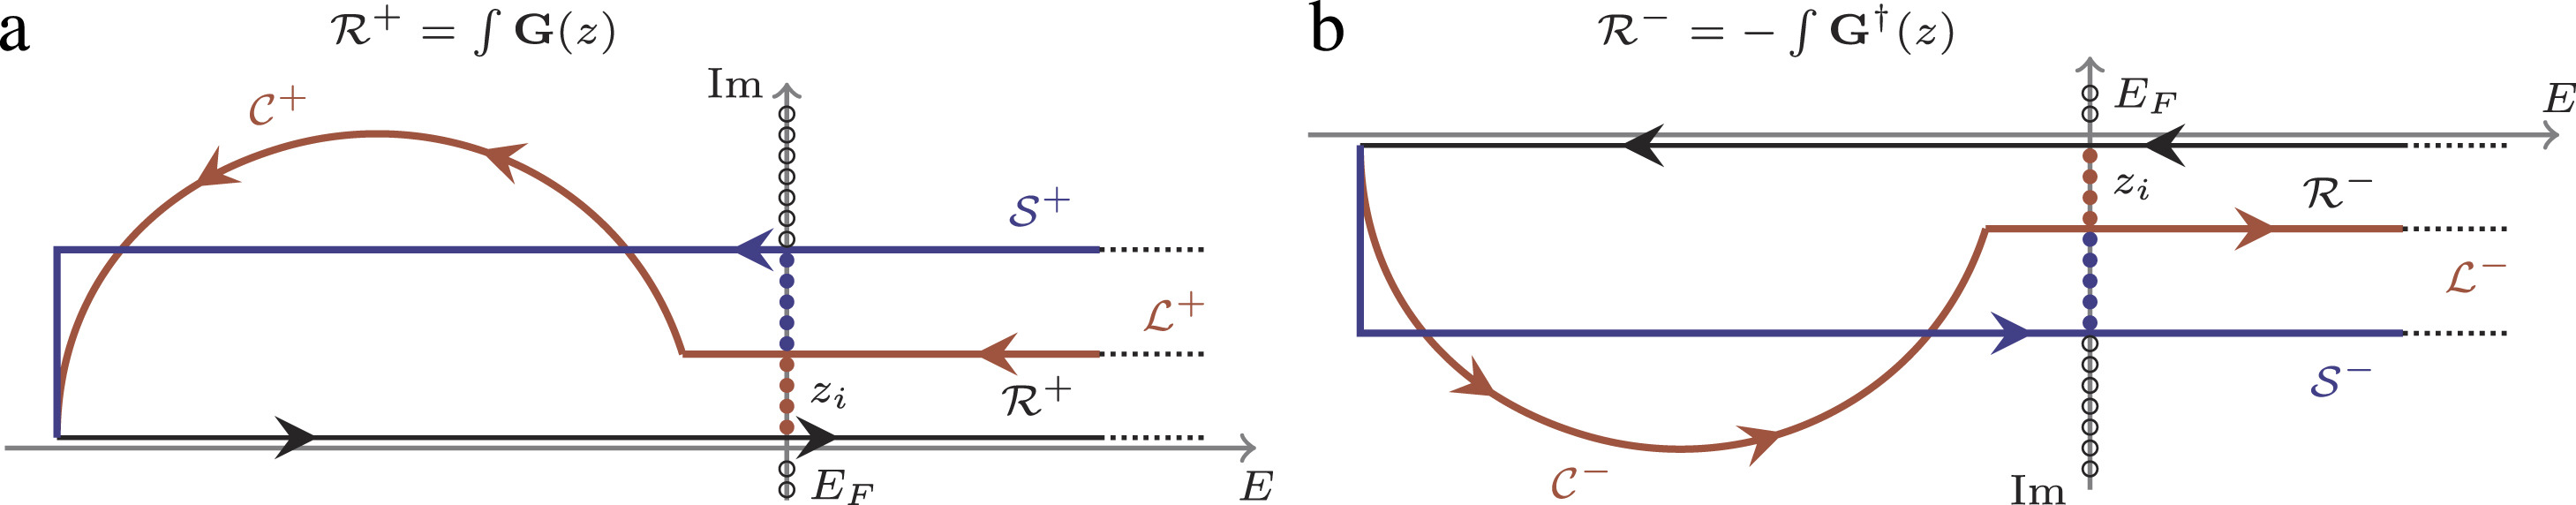
\includegraphics[scale=1]{figs/contour_green.jpg}
	 \legend{Fonte: \citeauthor{transiesta2}.}
	\label{fig:contour}
\end{figure} 

Por fim, o formalismo de NEGF+DFT pode ser encontrado no código \textit{Siesta} através da implementação do \textit{Transiesta}\cite{transiesta1,transiesta2,transiesta3}. A primeira versão do Transiesta foi publicada em \citeyear{transiesta1} e atualmente tem se destacado pela eficiência computacional e acurácia da estrutura eletrônica. Além disso, apresenta flexibilidade de simular situações mais realísticas, tais como a inclusão de defeitos em transporte eletrônico, a possibilidade de usar N>1 eletrodos e o cálculo de forças atômicas fora do equilíbrio \cite{transiesta4}. Em particular, o cálculo de forças permite realizar a otimização das coordenadas a fim de definir a posição de mínimo de acordo com o potencial externo aplicado. Assim, na seção seguinte apresentaremos como fazer o cálculo de forças em problemas fora do equilíbrio.


\subsection{Cálculo de Força Fora do Equilíbrio}
No estado fundamental e em sistemas independente do tempo, as forças que agem no núcleo de moléculas e sólidos podem ser obtidas pelo Teorema de Hellmann-Feynman (HF) \cite{forca-teo}\cite{forca-teo2}. Esse teorema estabelece que, dado uma hamiltoniana dependente de um parâmetro $ \lambda $ e sendo $ \Psi $ quadrado integrável, então, a força generalizada equivale à derivada da energia total em relação ao parâmetro $ \lambda $ (Equação \ref{eq:forca}). Esse teorema é válido tanto para funções de onda exatas ou expandidas em uma base finita.

\begin{equation}\label{eq:forca}
\vb{F}=-\dv{E}{\lambda}=-\underbrace{\flatfrac{\ev**{\pdv{H}{\lambda}}{\Psi}}{\braket{\Psi}{\Psi}}}_{\substack{\text{Força HF}}}-\underbrace{\flatfrac{\bqty{\mel**{\Psi}{H-E}{\pdv{\Psi}{\lambda}}-\mel**{\pdv{\Psi}{\lambda}}{H-E}{\Psi}}}{\braket{\Psi}{\Psi}}}_{\substack{\text{Força de Pulay}}}
\end{equation}

Onde, para $ \Psi $ exato\footnote{A forma convencional do teorema de HF é válido para funções de onda exatas ou expandidas em uma base finita, desde que: (a) as funções de base não dependam de $ \lambda $ ou (b) a derivada da base em relação à $ \lambda $ também faça parte da base. Essas regras são conhecidas por \textit{Condições de Hurley}.} a expressão se reduz à Força de HF e para uma base finita é acrescentado a correção de \textit{Pulay}. Para sistemas dependentes do tempo, $ \Phi=\Phi(t,\vb{r}) $, \citeauthor{force-teo3} propuseram uma definição mais geral do teorema de HF:
\begin{eqnarray}\label{eq:hf-geral}
\vb{F}=-i\hbar\dv{t}\ev**{\pdv{}{\lambda}}{\Phi}&=&-\flatfrac{\ev**{\pdv{H}{\lambda}}{\Phi}}{\braket{\Psi}{\Psi}}\nonumber\\&-&\flatfrac{\bqty{\mel**{\pdv{\Phi}{\lambda}}{H-i\pdv{t}}{\Phi}+\mel**{\Phi}{H+i\pdv{t}}{\pdv{\Phi}{\lambda}}}}{\braket{\Psi}{\Psi}}
\end{eqnarray}

Essa formulação é mais geral e vale para problemas de mecânica quântica fora do equilíbrio com estados estacionários, onde $ \ket{\Phi}=e^{-iEt/\hbar}\ket{\Psi} $. Assim, considerando o parâmetro $ \lambda=\vb{R_I} $  como a posição atômica do núcleo, então a Equação \eqref{eq:hf-geral} se reduz a:
\begin{equation}\label{eq:geral-red}
	\vb{F}_I=-\pdv{\ev{H}{\Psi}}{\vb{R}_I}
\end{equation}

Considerando que na DFT, o estado fundamental de energia é bem definido, de modo que as forças podem ser calculadas como a derivada da energia total com respeito à posição atômica $ \vb{R_I} $. Além disso, a força pode ser separada em duas contribuições:
\begin{equation}\label{eq:force-dft}
	\vb{F}=\vb{F}_{BS}+\vb{F}_{C}
\end{equation}
onde $ \vb{F}_{BS}=-\pdv{E_{BS}}{\vb{R_I}} $ corresponde à contribuição das energias das estruturas de banda e $ \vb{F}_{C} $ inclui as demais contribuições. Assim, considerando a equação de Kohn-Sham (Eq. \eqref{eq:kohn-sham}), o termo $ \vb{F}_{BS} $ equivale a:
\begin{equation}
	\vb{F}^{BS}=-\sum_{\mu\nu}D_{\mu\nu}\pdv{H_{\mu\nu}}{\vb{R}}+\Omega_{\mu\nu}\pdv{S_{\mu\nu}}{\vb{R}}
\end{equation}

onde $D_{\mu\nu}$ é a matriz densidade no equilíbrio e obtida por auto consistência e $\Omega_{\mu\nu}$ é a matriz densidade de energia:
$$\Omega_{\mu\nu}=\sum_i E_i f(E_i)\Psi_{i\mu}\Psi_{i\nu}$$

Como a Equação \eqref{eq:geral-red} é equivalente à \eqref{eq:forca}, e a partir dela a expressão \eqref{eq:force-dft} é obtida, logo ela também é válida para o caso de trasporte eletrônico com estado estacionário. Portanto, os termos $ D_{\mu\nu} $ e $ \Sigma_{\mu\nu} $ podem ser substituídos pelos equivalentes fora do equilíbrio, permitindo assim, calcular as forças atômicas no âmbito do formalismo NEGF+DFT. \cite{force-teo4}


\begin{comment}
\subsection{O código \textit{Transiesta}}
\todo[inline,color=green!40]{Falta mexer nessa parte}
O código Transiesta foi criado em 2002 por meio da implementação do formalismo de NEGF junto com DFT no código \textit{Siesta} pelos autores \citeauthor{transiesta1}. Atualmente, tem se destacado pela eficiência computacional, acurácia da estrutura eletrônica e flexibilidade de simular situações experimentais realísticas, tais como a inclusão de defeitos em transporte eletrônico e a possibilidade de usar N>1 eletrodos. Essas e outras melhorias constituíram o cerne das recentes modificações que o tem colocado em posição de destaque em simulações computacionais de transporte eletrônico \cite{transiesta2}\cite{transiesta3}\cite{transiesta4}. Em particular, a eficiência computacional está relacionado aos algoritmos de inversão utilizados para resolver o produto de matriz triplo. Assim, nessa seção será apresentado o principal algoritmo de inversão utilizado no Transiesta \textit{Block-tri-diagonal}(BTD). 

A utilização de bases atômicas localizadas faz com que as matrizes Hamiltoniana, de densidade e de \textit{overlap} sejam esparsas. Para calcular as funções de Green na situação fora do equilíbrio, é necessário obter a matriz inversa dessas matrizes tridiagonais (incluindo as autoenergias) por meio de algoritmos especializados em inversão com elementos não nulos concentrados em certas posições. Na Figura \ref{fig:matriz}, vemos uma representação ilustrativa dos blocos de matrizes (Eq. \eqref{eq:matriz-esparsa}) que descrevem os eletrodos e a região de espalhamento da abordagem típica de um problema de transporte eletrônico \cite{exemplo}, onde os blocos maiores representam os eletrodos e os menores a região de espalhamento.

\begin{figure}[h!]
	\centering
	\includegraphics[scale=0.3]{figs/matriz_esquema.png}
	\caption{\textit{Esquema ilustrativo das matrizes tridiagonais que descreve um sistema de transporte eletrônico. Fonte: \citeauthor{exemplo}.}}
	\label{fig:matriz}
\end{figure}  

De acordo com esse algoritmo, dado uma matriz tridiagonal $ \vb{M} $, no qual as matrizes que compõem a diagonal ($ \vb{A_1} $ a $ \vb{A_N} $) são quadradas e invertíveis \cite{algoritmo}.

\begin{equation}
	M=\begin{bmatrix}
		\vb{A_1} & \vb{C_2} & 0 & \cdots  & 0 \\ 
		\vb{B_1} & \vb{A_2} & \vb{C_3} & \cdots  & 0\\ 
		0 & \vb{B_2} & \vb{A_3} & \cdots  &0 \\ 
		\vdots  & \vdots  & \vdots  & \vdots  & \vdots \\ 
		0& 0 &0  & 0 & \vb{A_N}
	\end{bmatrix}
\end{equation}
então, os blocos diagonais de $ \vb{M}^{-1} $ são dados por:
\begin{equation}
	(\vb{M}^{-1})_{n,n}=\bqty{\vb{A}_n-\vb{X}_n-\vb{Y}_n}^{-1}
\end{equation}
onde, 
\begin{equation}\label{eq:btd1}
	\vb{X_N}=\left\{\begin{matrix}
		0 & \text{se}\quad n=N\\ 
		\vb{C_{n+1}}\bqty{\vb{A}_{n+1}-\vb{X}_{n+1}}^{-1}\vb{B}_n &\text{se}\quad1\leq m< N 
	\end{matrix}\right.
\end{equation}

\begin{equation}\label{eq:btd2}
	\vb{Y_N}=\left\{\begin{matrix}
		0 & \text{se}\quad n=1\\ 
		\vb{B}_{n-1}\bqty{\vb{A}_{n-1}-\vb{Y}_{n-1}}^{-1}\vb{C}_n &\text{se}\quad1\leq m< N 
	\end{matrix}\right.
\end{equation}

Os termos fora da diagonal são dados por:

\begin{equation}
	(\vb{M}^{-1})_{m,n}=\left\{\begin{matrix}
		-\bqty{\vb{A}_m-\vb{X}_m}^{-1}\vb{B}_{m-1}(\vb{M}^{-1})_{m-1,n} & \text{se}\quad m>n\\ 
		-\bqty{\vb{A}_m-\vb{X}_m}^{-1}\vb{C}_{m-1}(\vb{M}^{-1})_{m+1,n} & \text{se}\quad m<n
	\end{matrix}\right.
\end{equation}
 
Associando esse método ao cálculo das funções de Green fora do equilíbrio, podemos equiparar a matriz $ \vb{G}^{-1} $ à matriz $ \vb{M}^{-1} $, onde as matrizes $ \vb{A}_i,\vb{B}_i $ e $ \vb{C}_i $ correspondem aos elementos não nulos de $ \epsilon\vb{S}-\vb{H}-\vb{\Sigma}_L-\vb{\Sigma}_R $. Na Figura \ref{fig:btd} está ilustrado como os termos que compões a inversa da matriz são obtidos recursivamente. Além disso, vemos que o termo $ \vb{Y}_1 $ resulta na autoenergia do eletrodo esquerdo ($ \Sigma_1 $) e $ \vb{X}_1 $ ao eletrodo direito. 

\begin{figure}[h!]
	\centering
	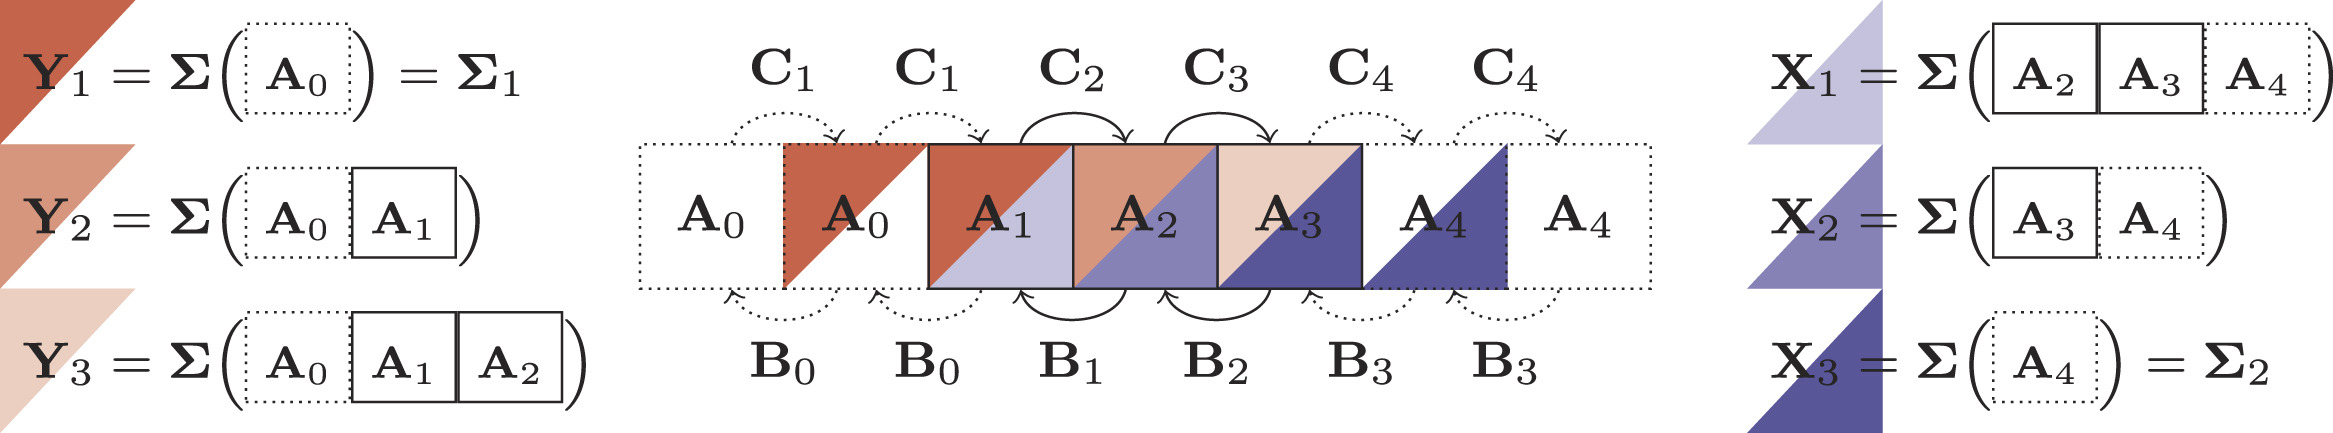
\includegraphics[scale=1.25]{figs/btd.jpg}
	\caption{\textit{Fonte: \citeauthor{transiesta2}.}}
	\label{fig:btd}
\end{figure} 

Dessa forma, considerando que a inversa de $ \vb{G}^{-1} $ é em princípio definida, é possível calcular os termos $ \vb{Y}_n $ e $ \vb{X}_n $ e com isso, aplicar novamente o algoritmo de inversão sobre $ \vb{G}^{-1} $ é possível calcular, de fato, $ \vb{G} $. Aplicando as equações \eqref{eq:btd1} e \eqref{eq:btd2}, obtemos as equações para $ \vb{G} $ como ilustrado na Figura \ref{fig:btd2}. Assim, esse método facilita o cálculo do produto matricial triplo da matriz densidade fora do equilíbrio. Por fim, na Figura \ref{fig:btd2} está ilustrado a performance do algoritmo BTD em comparação aos algoritmos de inversão LAPACK e MUMPS para o cálculo da matriz no equilíbrio (a) e fora do equilíbrio (b).  \cite{transiesta3}

\begin{figure}[h!]
	\centering
	\includegraphics[scale=2.0]{figs/performance.jpeg}
	\caption{\textit{Fonte: Comparação da performance dos códigos LAPACK e MUMPS em relação ao BTD na solução dos contornos no equilíbrio (a) e fora (b) para uma estrutura de grafeno composta por 24 átomos. \citeauthor{transiesta2}.}}
	\label{fig:btd2}
\end{figure} 


\begin{comment}
\section{Funções de Green no Equilíbrio\label{cap:fora}}

As funções de Green são definidas como as soluções de equações diferenciais inomogêneas, cuja expressão é dada por:
$$
    \bqty{z-L(\vb{r})}\green=\delta(\vb{r}-\vb{r'})
$$
sujeito à condições de contorno situadas na superfície $S$ do domínio $\Omega$ de $\vb{r}$ e $\vb{r'}$. De acordo com a notação utilizada, $z$ é uma variável complexa com $\lambda\equiv Re\Bqty{z}$ e $s\equiv Im\Bqty{z}$ e $L(\vb{r})$ é um operador diferencial linear, hermitiano e que possui um conjunto de autofunções $\Bqty{\varphi_n(\vb{r})}$ que satisfazem as mesmas condições de contorno que $\green$ \cite{green}. Para obter as propriedades das Funções de Green, é mais conveniente reescrever a equação acima utilizando a notação de Dirac:
\begin{eqnarray}\label{eq:dirac}
    \pqty{z-L}G(z)&=&\mathbb{1}\delta(z)\qquad\text{onde,}\\
    \quad\green&\equiv&\mel{\vb{r}}{G(z)}{\vb{r'}}\nonumber
\end{eqnarray}

A partir da definição de Funções de Green, podemos abordar o caso de partículas livres, cuja equação é dada por:
\begin{equation}\label{eq:livre}
    i\hbar\pdv{t}\ket{\Psi_0(t)}=\mathnormal{H}_{0}\ket{\Psi_0(t)}
\end{equation}
 Onde $H_0$ representa a energia cinética das partículas. Podemos escrever essa equação em termos de um operador diferencial linear $L=i\hbar\pdv{}{t}-H_0$, de modo que:
 \begin{equation}
     L\ket{\Psi_0(t)}=f(t)\qquad\text{com}\;f(t)=0
 \end{equation}
 
 Assim, podemos associar à Equação \ref{eq:livre} dois tipos de funções de Green $G_0^r(t)$ e $G_0^r(t)$, de modo que a Equação \eqref{eq:dirac} resulta em:
 \begin{equation}
     LG_0^{r,a}(t)=\pqty{i\hbar\pdv{}{t}-H_0}G_0^{r,a}(t)=\mathbb{1}\delta(t)
 \end{equation}
 com as seguintes condições de contorno:
 \begin{eqnarray}
     G_0^r(t)&=&0,\qquad t<t_0=0\\
     G_0^a(t)&=&0,\qquad t<t_0=0
 \end{eqnarray}
 
Aplicando essas condições de contorno, as soluções das equações de movimento são dadas por:
\begin{eqnarray}
\begin{aligned}G_{0}^r(t)&=\begin{cases}
 \;-\frac{i}{\hbar}e^{-iH_0t/\hbar},\qquad& t>t_0=0\\
  \quad 0\;,\quad &t<t_0=0
\end{cases}\end{aligned}\\\begin{aligned}
 G_{0}^a(t)&=\begin{cases}
   \quad 0 \;,\quad &t>t_0=0 \\
  \quad \frac{i}{\hbar}e^{-iH_0t/\hbar},\qquad & t<t_0=0\end{cases}\end{aligned}
\end{eqnarray}

Para a condição $t>t_0=0$, $G^r_0(t)$ é proporcional ao operador de evolução temporal $U(t,t_0=0)=e^{iH_0(t-t_0)/\hbar}=e^{-iH_0t/\hbar}$. Assim, a função de Green $G^r_0(t)$ pode ser associada ao propagador do temporal do estado $\ket{\Psi_0(t)}$ de $t_0$ a $t$, sendo, portanto denominada como função de Green retardada.
\begin{equation}
    \ket{\Psi_0(t)}=i\hbar G^r_0(t,t_0)\ket{\Psi_0(t_0}
\end{equation}

Da mesma forma, para $t<t_0$, a função de Green $G^a_0(t)$ é denominada como função de Green avançada, pois relaciona o estado $\ket{\psi_0(t_0)}$ com o estado passado $\ket{\psi_0(t)}$ e atua como um propagador desse estado de um tempo $t$ no passado, até o presente $t_0$.

\begin{equation}
    \ket{\Psi_0(t)}=-i\hbar G^a_0(t,t_0)\ket{\Psi_0(t_0}
\end{equation}
\section{O Código Smeagol\label{cap:cod}}
\end{comment}